\documentclass[a4paper,10pt,twoside]{article}
\pdfoutput=1 
\usepackage[bookmarks=true]{hyperref}

\usepackage{bookmark}
\bookmarksetup{
  numbered, 
  open,
}


\usepackage{todonotes}
\usepackage{amssymb,amsmath}       % Equations
\usepackage{array}
\usepackage{bm}                    % Bold math symbols
\usepackage{epsfig}
\usepackage{float}
\usepackage{graphicx,color,psfrag} % Graphics, Figures
\usepackage{tikz}
\usepackage{multirow}              % For Tables
\usepackage{tabularx}              % Tables
\usepackage{wrapfig}
\usepackage[algoruled]{algorithm2e}
\SetStartEndCondition{ }{}{}%
\SetKwProg{Fn}{def}{\string:}{}
\SetKwFunction{Range}{range}%%
\SetKw{KwTo}{in}\SetKwFor{For}{for}{\string:}{}%
\SetKwIF{If}{ElseIf}{Else}{if}{:}{elif}{else:}{}%
\SetKwFor{While}{while}{:}{}%
% \renewcommand{\forcond}{$i$ \KwTo\Range{$n$}}
\AlgoDontDisplayBlockMarkers\SetAlgoNoEnd\SetAlgoNoLine%


%% enumitem 
% \labelindent is defined in both IEEEtrans and
% enumitem. \let\labelindent\relax kind-of disables \labelindent
% defined in IEEEtrans, hence avoiding the name clash.
\let\labelindent\relax
\usepackage[inline]{enumitem}

%% algorithm2e
% \usepackage[plain]{algorithm2e}
% remove line number for one line
% \let\oldnl\nl
% \newcommand{\nonl}{\renewcommand{\nl}{\let\nl\oldnl}}

%% subfigure
\usepackage[caption=false,font=footnotesize]{subfig}
% make references to subfigures appear as \thefigure(\thesubfigure)
\captionsetup[subfigure]{subrefformat=simple,labelformat=simple,listofformat=subsimple}
\renewcommand\thesubfigure{(\alph{subfigure})}

% variables
\newcommand{\mc}[2][]{{\mathcal{#2}_{\textrm{#1}}}}
\newcommand{\q}[1]{\bm{q}_{\textrm{#1}}}
\newcommand{\qd}[1]{\bm{\dot{q}}_{\textrm{#1}}}
\newcommand{\T}[1]{\bm{T}_{\textrm{#1}}}
\newcommand{\x}[1]{\bm{x}_{\textrm{#1}}}
\newcommand{\qvect}{\bm{q}}
\newcommand{\Tvect}{\bm{T}}
\newcommand{\GP}{\mathcal{G}\cap\mathcal{P}}
\newcommand{\cP}{\mathcal{P}}
\newcommand{\cC}{\mathcal{C}}
\newcommand{\cO}{\mathcal{O}}
\newcommand{\bfp}{\mathbf{p}}
\newcommand{\calT}{\mathcal{T}}
\DeclareMathOperator*{\argmin}{arg\,min}
\DeclareMathOperator*{\argmax}{arg\,max}
% acronyms
\newcommand{\ie}{{\textit{i.e.}}}
\newcommand{\etal}{\textit{et~al.}}

% theorem environment
\newtheorem{theorem}{Theorem}
\newtheorem{proof}{Proof}
\newtheorem{lemma}{Lemma}
\newtheorem{proposition}{Proposition}
\newtheorem{corollary}{Corollary}
\newtheorem{remark}{Remark}
% TODO
\newcommand{\TODO}[1]{\noindent {\color{red} \{{\bf To-do:} #1\}}}
% COMMENT
\newcommand{\comment}[1]{}

% change tt font
\renewcommand{\tt}{\fontfamily{cmtt}\selectfont}

% figures path
\graphicspath{{figures/}}

% \overrideIEEEmargins
% set margins
\setlength{\floatsep}{2pt plus 1pt minus 1pt}
\setlength{\textfloatsep}{5pt plus 1pt minus 2pt}

%% TITLE
\title{MAS714-Homework 2}
%% AUTHOR
\author{Pham Tien Hung, Zhang Xu
}

%% DATE
\date{}


%%%%%%%%%%%%%%%%%%%%%%%%%%%%%%%%%%%%%%%%%%%%%%%%%%%%%%%%%%%%%%%%%%%%%%
\begin{document}
\maketitle
\listoftodos[Notes]

\section*{Exercise 1}
\subsection*{a)}
\begin{proposition}
Every tree is a bipartite graph.
\end{proposition}
\begin{proof}
	We will prove by induction, that is very tree $T(V, E)$ whose
	$|V| = n$ for all $n$ is a bipartite graph. The case $n=2$ is trivially true.

	Assume that this is true for $|V| = n$, we will now prove that it
	is true for every tree $T'$ whose $|V'| = n + 1$. 

	Consider one such tree $T'$ with $|V'| = n + 1$, we select a leaf node $u$
	and remove it from $T'$ creating $T''$. Clearly, $|V''| = n$ and
	therefore $T''$ is now a bipartite graph. Let $L''$ and $R''$ be the
	corresponding bipartite set of the tree $T''$.

	Without loss of generality, assume that the node $u$ connects to
	some node $v$ belonging to $L''$, we construct two new set $L'$
	and $R'$:
	\[
		L' = L''
	\]
	\[
		R' = R'' \cup \{u\}
	\]
	Clearly, this is enough to say that $T'$ is bipartite.	
\end{proof}

\subsection*{b)}
\begin{algorithm}[H]
	\caption{Check for bipartite graph ($G(V, E)$)}
	$T$, $BE$ = DFS(G) \tcp*{$BE$ is the list of back edges}
	Let bipartite = True\;
	\For{edge $(u, v)$ in $BE$}{
		\If{$\|pre(v) - pre(u)\|$ is even}{
			bipartite = False \tcp*{The cycle containing $(u, v)$ has odd number of edges}
		}
	}
	\Return bipartite
\end{algorithm}
\subsubsection*{Analysis of complexity}
The algorithm is essentially the same as DFS, therefore its complexity is $O(n + m)$.

\subsubsection*{Proof of correctness}
We first state three propositions.
\begin{proposition}
	Given a connected graph $G$, $G$ is bipartite iff any cycles in $G$ have even number of
	edges.
\end{proposition}
\begin{proof}
	The first direction is trivial. If $G$ is bipartite, then every cycle in $G$
	must have even number of edges. 

	To see this is true, assume the contradition,
	that is there exists a cycle with odd number of edge: $v_1,...,v_n$ for $n$ odd. 
	Since every odd number vertex is connected with an even number vertex, we must
	separate the vertices into odd-set and even-set. However, $v_1$ and $v_n$ also connects
	which implies that $G$ is not bipartite.

	Now, we must show that if every cycle in $G$ has even number of edge, then $G$ is
	bipartite. 
	To do this, we first find a spanning tree $T$ from $G$ using DFS; then, we divide $T$
	into two set $R$ and $L$. Then we will show that all edges in the set of back edges
	$E\setminus T$ connects one vertex in $R$ and one vertex in $L$.

	Consider one such back edge $(u, v)$, assuming we add this edge into the tree $T$.
	Clearly, we will obtain a cycle with even number
	of edges $u, v_1, v_2, ..., v_n, v$ in $T \cup \{(u, v)\}$. Now, assuming w.l.g that
	$u\in R$, clearly $v_1 \in L$ and so on, which will lead to $v \in L$ due to eveness
	of the number of vertices/edges.

	Repeat this procedure for all edges in $E\setminus T$. The proof follows.



\end{proof}
\begin{proposition} 
	Given a graph $G(V, E)$, if all cycles discovered by DFS
	have even number of edges then all cycles in $G$ have even number of edges.
\end{proposition}
\begin{proof}
	To prove this proposition, we first define a notion of combining cycle with cycle.
	Assuming we have two cycles with a common sequence of vertices
	\[
		v_i,...,v_j,v_a,...,v_b,v_k,...,v_i
	\]
	\[
		v'_i,...,v'_j,v_a,...,v_b,v'_k,...,v'_i	
	\]
	where $v_a, ..., v_b$ is the same for both cycle. We can then form a new cycle
	\[
		v_i,...,v_j,v_a,v'_j,...,v'_i,...,v'_k,v_b,v_k,...,v_i	
	\]

	It is trivial to show that two cycles with even number of edges combine to form a cycle
	with even number of edge. Another thing to note is that in the new cycle, the edges
	between $v_a,...,v_b$ are deleted.

	Additionally, if two cycles are exactly the same, then their combination is the the empty set $\emptyset$.

	Now we will prove the main proposition by contradition. That is, suppose all cycles found
	by DFS have even number of edges, there exist a cycle with odd number of edges. Let this cycle
	be $C_o$, $C_o$ must contains some back edges, otherwise it will not be a cycle. We combine
	$C_o$ with the cycles corresponding to the back edges which $C_o$ has. At the moment when 
	$C_o$ consists of only one back edge, its number of edge is odd. We now combine $C_o$ with
	the cycle (found with DFS) containing the last back edge to form yet another cycle. This cycle
	does not contains any back edge.

	Note that this combination can't become $\emptyset$ because $C_o$ and 
	the last cycle are different (one has odd, one has even number of edge).

	Having a cycle without any back edge leads to a contradition.

\end{proof}
\begin{proposition}
	Given a graph $G(V, E)$, let us apply DFS on $G$. Considering a back-edge $(u, v)$, then
	$\|pre(v) - pre(u)\|$ is odd iff the number of edges in the cycle discovered by DFS is even. 
\end{proposition}
\begin{proof}
	To show that this is correct, we simply note that in a DFS tree, if $v$ is the direct child
	of $u$ then $$(pre(v) - pre(u))$$ is always odd.

	Now, we construct a cycle from a DFS tree by going to one node's direct parent, therefore
	it is clearly that for all nodes in a cycle discovered by DFS the above relationship holds.

	The proof follows simply.
\end{proof}
\begin{proposition}
	Algorithm 1 is correct.
\end{proposition}

\begin{proof}
	The proof follows from the three above proposition via direct equivalences.
\end{proof}



\section*{Exercise 2}

Assume that $X_L[1...n]$ is sorted with $X_L[1]$ being the smallest member.

\begin{algorithm}[h]
\caption{Find maximum tiling ($X$)}
	Let $x$ be $-\infty$ \;
	Initialize $T = \emptyset$\;
	\While{$X$ is not empty}{
		\eIf {$X_L[0] > x$}{
			Let $x_{stop} = X_L[0]$\;
		}{Let $x_{stop} = x$}
		Let $x_{max} = -\infty$\;
		\While{$X_L[0] \leq x_{stop}$}{
			\If {$X_R[0] > x_{max}$}{
				$x_{max} = X_R[0]$\;
				Select $X[0]$ as the chosen interval $i$\;
			}
			Remove $X[0]$ from $X$\;
		}
		Add the selected interval $i$ to $T$\;
		% Let $O$ be the set of interval such that $X_L[i] \leq x$\;
		% \If {$O == \emptyset$}{
		% 	Let $O$ be the set of interval such that $X_L[i] == X_L[0]$\;
		% }
		% Let $X = X \setminus O$\;
		% Sort $O$ according to the right end point\;
		% Let $y = \argmax_{i \in O} i_R$\;
		% Let $T = T\cup\{y\}$\;
		% Let $x = y_R$\;
	}
	\Return $T$\;
\end{algorithm}

\subsubsection*{Analysis}
Running time $O(n)$.
\todo{Analyze exercise 2's algorithm}
\subsubsection*{Proof of correctness}
\todo{Complete the proof for exercise 2}
\section*{Exercise 3}

\subsection*{a}
Not all Minimum Bottleneck Tree (MBT) is a MST. Here is a counter example:

\begin{figure}[h]
	\centering
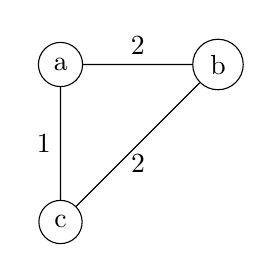
\begin{tikzpicture}
	\path 	(0, 2) node[circle, radius=2.5pt, draw] (a) {a}
			(2, 2) node[circle, radius=2.5pt, draw] (b) {b}
			(0, 0) node[circle, radius=2.5pt, draw] (c) {c};
	\draw (a) 
				-- node[above] {2} (b) 
				-- node[below] {2} (c) 
				-- node[left] {1} (a);
\end{tikzpicture}
	\label{fig:figure1}
\end{figure}
The tree containing two edges $(a, b), (b, c)$ is an MBT but is clearly
not a MST.

\subsection*{b}
\begin{proposition}
We will show that given an undirect graph $G$ with distinct edge
cost, if $T$ is $G$'s minimum spanning
tree (MST) then it is also a minimum-bottleneck tree (MBT) of $G$.	
\end{proposition}
\begin{proof}
	We will prove by contradition. That is, let $T$ be an MST of $G$,
	there must exist a spanning tree $T'$ whose maximum edge cost
	being smaller than the maximum edge cost of $T$.
	Let $e_i$ and $e'_i$ denote the edges of $T$ and $T'$ respectively.
	This means
	\[
		\max_i{e'_i} < \max_i{e_i}.
	\]

	Let the maximum edge of $T$ be $e_j$, we thus have
	\[
		\forall i, e'_i < e_j.
	\]

	Now consider the cut $(S, V\setminus S)$ that $e_j$ is the corresponding
	safe edge, there must exist an edge $e'_j$ in $T'$ that also crosses $(S, V\setminus S)$.
	We thus have
	\[
		e'_j < e_j \leq e'_j
	\]
	which is clearly a contradition.
\end{proof}
\section*{Exercise 4}
\begin{proposition}
\label{prop:4-1}
	Let $T$ be the MST of $G(V, E)$, assuming we add a new edge $c$ to $G(V, E)$, the
	MST of the modified graph must be a subset of $T\cup \{c\}$.
\end{proposition}
\begin{proof}
	We will prove by contradiction. That is the MST of the modified graph contain some $e_i$ which
	does not belong to $T \cup \{c\}$. Suppose $e_i$ is the safe edge crossing some cut 
	$(S, V\setminus S)$ of the graph $G'(V, E \cup \{c\})$. Suppose $e_j$ is the safe edge
	crossing $(S, V\setminus S)$ of the graph $G(V, E)$. Clearly:
	\[
		e_i \neq e_j, e_i \neq c
	\]

	Now, let $E(S, V\setminus S)$ and $E'(S, V\setminus S)$ be the set of edges crossing
	the said cut in two graphs $G$ and $G'$ respectively. There are only two cases: 
	1) 
	$$E'(S, V\setminus S)=E(S, V\setminus S) \cup \{c\}$$ and 2) 
	$$E'(S, V\setminus S)=E(S, V\setminus S)$$
	In both case, $e_i \neq e_j, e_i \neq c$
	lead to contradition.

\end{proof}

\begin{proposition}
\label{prop:4-2}
	Let $T$ be the MST of $G(V, E)$. Suppose we remove some edges which do not belong
	to $T$ from $G$, then $T$ is also the MST of the modified graph.
\end{proposition}
\begin{proof}
	We will prove this by showing that every safe edge of $G$ must also be a safe edge
	of the modifed graph $G'$. Clearly, let's assume $e_i$ is a safe edge of $G$ crossing a cut
	$(S, V\setminus S)$. Since we do not remove safe edge from $G$ to create $G'$, clearly
	$e_i$ also crosses the same cut in the modifed graph $G'$. This implies $e_i$ is also
	a safe edge of $G'$.
\end{proof}


\subsection*{a}

\begin{algorithm}[H]
	\caption{Check for MST($G, T, c$)}
	Let $P=(e_1, ..., e_n)$ be the cycle computed with DFS($T \cup \{c\}$)\;
	\eIf{$c$ is the edge with largest cost in $P$}{
		\Return False \tcp*{$T$ remains the MST}
	}
	{
		\Return True \tcp*{$T$ does not remain the MST}
	} 

\end{algorithm}

Complexity $O(n)$ since it is dominated by DFS algorithm.

\begin{proposition}
	Given a graph $G$, let's $T$ be the MST of $G$. Suppose we add a new edge
	$c$ to $G$ to create $G'$. Then $T$ remains the MST of $G'$ iff $c$ is the
	edge with largest cost in the cycle containing $c$ in the graph $T\cup \{c\}$.
\end{proposition}
\begin{proof}
	Let's $T'$ be the MST of $G'$. Acoording to proposition~\ref{prop:4-1},
		\[
		 	T' \subset T \cup \{c\}
		 \]
	Clearly, $T\cup \{c\}$ can be created by removing non-MST edge from $G'$, therefore
	according to proposition~\ref{prop:4-2}, $T'$ must the be MST of $T \cup \{c\}$.

	Now, $T' = T$ is equivalent to $c$ being an unsafe edge in the graph $T \cup \{c\}$.
	This is in turn equivalent to $c$ being the
	edge with largest cost in some cycles containing $c$ in the graph $T\cup \{c\}$.

	Now, since $T$ is a tree, there can be only one simple cycle in $T\cup \{c\}$ and 
	the cycle contains $c$. The proof follows.

\end{proof}
\subsection*{b}
\begin{algorithm}[H]
	\caption{Fix MST($G, T, c$)}
	Let $P=(e_1, ..., e_n)$ be the cycle computed with DFS($T \cup \{c\}$)\;
	Let $e_m = \max_{i\in P} e_i$\;
	\Return $T \cup \{c\} \setminus \{e_m\}$ 

\end{algorithm}

Complexity $O(n)$ since it is dominated by DFS algorithm.

\begin{proposition}
	Given a graph $G$, let's $T$ be the MST of $G$. Suppose we add a new edge
	$c$ to $G$ to create $G'$. Then we can compute $T'$--the MST of $G'$--by looking
	for the edge with largest cost in the graph $T\cup \{c\}$.
\end{proposition}
\begin{proof}
	Following similar arguments as the proof for part a, we see that $T'$ must be
	the MST of $T \cup \{c\}$. The edge with maximum cost is therefore an unsafe edge
	and its removal would result in the set of only safe edges. 

	The proof follows.	
\end{proof}


\section*{Exercise 5}
\begin{algorithm}[H]
	\caption{Algorithm($G(V, E)$)}
	Initialize new set of vertices $V' = V$\;
	Initialize new set of edges $E' = \emptyset$\; 
	\For{$e_i$ in $E$}{
		add new edge $e'_i = -\log (1 - e_i)$ to $E'$
	}
	\Return Dijkstra($G'$)
\end{algorithm}

\subsubsection*{Analysis}
This algorithm complexity is basically the same as Dijkstra, which is 
$$O((n + m)\log n)$$

\subsubsection*{Proof of correctness}
We will show that if a set of edge $(e_1, e_2, ..., e_k)$ has the lowest
negated logarithmic cost then they have the least chance of at least
one edge failed.

Additionally, it is remarked that the negated logarithmic cost is always
positive. This ensures Dijkstra works correctly.

\begin{proof}
	Given some edge $(e_i,...)$, let the chance of having at least one failure
	be $R_f$ and the chance of all edge success be $R_s$, we have:
	\[
	 	R_f + R_s = 1
	 \] 
	 where $R_s = \prod_i{1-e_i}$.

	 Since $P = \{e_i,...\}$ has the lowest negated log cost, for any 
	 other path $P' = \{e_j,...\}$
	 we have the following
	 \[
	 	\begin{aligned}
	 		- \sum_{e_i \in P}{\log{(1 - e_i)}} &\leq - \sum_{e_i \in P'}{\log{(1 - e_i)}} \\
	 		\sum_{e_i \in P}{\log{(1 - e_i)}} &\geq \sum_{e_i \in P'}{\log{(1 - e_i)}} \\
	 		\prod_{e_i \in P}{(1 - e_i)} &\geq \prod_{e_i \in P'}{(1 - e_i)} \\
	 		R_s(P) & \geq R_s(P') \\
	 		R_f(P) & \leq R_f(P') \\
	 	\end{aligned}
	 \]
\end{proof}
\end{document}
